\documentclass{beamer}
%\usetheme{Warsaw}
\usepackage{color}
\usepackage{lmodern}
\usepackage[T1]{fontenc}
\usepackage[utf8x]{inputenc}
\usepackage[ngerman]{babel}
\usepackage{graphicx}
%\usepackage{inconsolata} % TT font
\usepackage{amsmath}
\usepackage{amsfonts}
\usepackage{textcomp}
\usepackage{hyperref}
\usepackage{url}
\usepackage{array}

\title{Suffix Arrays und BWT}
\author{Tobias Harrer}
\date{19.11.12}
 
\begin{document}
\maketitle
%\frame{\tableofcontents[currentsection]}
 
\begin{frame}
\tableofcontents
\end{frame} 
 
\section{Suffix Arrays}
%%%%%
\subsection{Grundlagen}
\begin{frame} %%Eine Folie
  \frametitle{Suffix Arrays} %%Folientitel
  \begin{Definition} %%Definition
  \begin{itemize}
  \item Sei T ein String der Länge n über $\Sigma$ und $T_{i,j}$ mit $(0<i\leq j\leq n)$ der Substring von i bis einschließlich j, dann ist $T_{i,n}$ ein Suffix von T.
  \item Das Suffix Array von T ist die Permutation der Startindizes i der lexikografisch geordneten Suffixes $T_{i,n}$ von T.
  \item Anmerkung: jeder String T endet mit \$, s.d für alle $c \in \Sigma$ gilt $\$ < c$ 
  \end{itemize}
  \end{Definition}
\end{frame}
\begin{frame}
\frametitle{Suffix Arrays - Beispiel} %%Folientitel
T = \glqq abacabra\$\grqq\\[5mm]

\begin{tabular}{r|l<{\ttfamily} r<{\ttfamily}}
\textbf{i $T_{i,n}$} & \textbf{lexikografisch geordnet}\\\hline
1 & abacabra\$ & \$ 9\\
2 & bacabra\$ & a\$ 8\\
3 & acabra\$ & abacabra\$ 1\\
4 & cabra\$ & abra\$ 5\\
5 & abra\$ & acabra\$ 3\\
6 & bra\$ & bacabra\$ 2\\
7 & ra\$ & bra\$ 6\\
8 & a\$ & cabra\$ 4\\
9 & \$ & ra\$ 7\\
\end{tabular}\\[5mm]
Das Suffix Array von T lautet: \newline
{\ttfamily
\qquad 1 2 3 4 5 6 7 8 9 \textrightarrow\ \textbf{i}\newline
\qquad 9 8 1 5 3 2 6 4 7 \textrightarrow\ \textbf{A(i)}
}
\end{frame}
%%%%
\subsection{Suffix Arrays aus Suffix Trees}
\begin{frame}
\frametitle{Suffix Arrays aus Suffix Trees} %%Folientitel
\begin{itemize}
\item Sortierung durch z.B. mergeSort in $\mathcal{O}(n\cdot log (n))$
\item Suffix Array kann aus Blättern eines Suffix Trees durch Tiefensuche hergeleitet werden: T = \glqq abacabra\$\grqq\newline
\end{itemize}
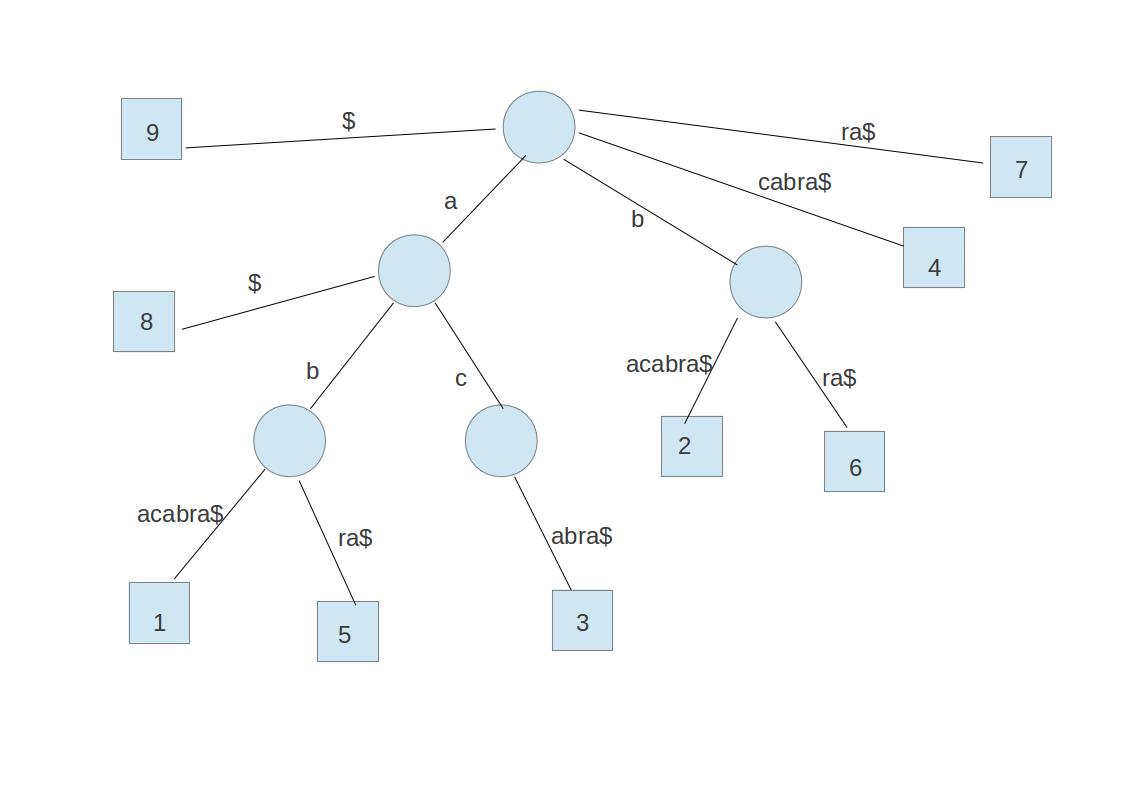
\includegraphics[scale=0.28]{SuffixTree.jpg}%[height=0.5\textheight]
\end{frame}
%%%%
\subsection{Anwendung von Suffix Arrays}
\begin{frame}
\frametitle{Anwendung von Suffix Arrays}
\begin{itemize}
\item Finde Pattern p (\glqq cab\grqq) in String T (\glqq abacabra\grqq)
\item Naiver Ansatz: \glqq schiebe\grqq\ p über T: \newline
{\ttfamily
abacabra \newline
cab\textrightarrow \newline
...\newline
abacabra \newline
. . cab
}
\item Problem: $\mathcal{O}(n\cdot m)$
\end{itemize}
\end{frame}
%
\begin{frame}
\frametitle{Anwendung von Suffix Arrays}
\begin{itemize}
\item Vorteil: alle Suffixes lexikografisch sortiert
\item p \glqq abr\grqq ist Präfix $T_{1,3}$ des Suffix $T_{5,n}$: \newline
\begin{tabular}{r|l<{\ttfamily}}
\textbf{A[i]} & \textbf{$T_{A[i],n}$}\\\hline
9 & \$\\
8 & a\$\\
1 & abacabra\$\\
5 & {\color{red}\textbf{abr}}a\$\\
3 & acabra\$\\
2 & bacabra\$\\
6 & bra\$\\
4 & cabra\$\\
7 & ra\$\\
\end{tabular}
\item Beste Suchstrategie in sortiertem Array?
\end{itemize}
\end{frame}
%%%%%%%%%%%%Beginn erster Bsp. Suche von "abr"		%%%%%%%%%%%
\begin{frame}
\frametitle{Anwendung von Suffix Arrays}
\begin{itemize}
\item Binäre Suche, Vergleich von \glqq abr\grqq mit $T{A[i],A[i]+2}$:\newline
\begin{tabular}{l|l<{\ttfamily}}
\textbf{A[i]} & $T_{A[i],n}$\\\hline
9 & \$\\
8 & a\$\\
1 & abacabra\$\\
5 & abra\$\\
3 & \color{red}\textbf{aca}\color{black}bra\$\ \glqq abr\grqq $<$ \color{red}\glqq aca\grqq \color{black}\textrightarrow obere Hälfte\\
2 & bacabra\$\\
6 & bra\$\\
4 & cabra\$\\
7 & ra\$\\
\end{tabular}
\end{itemize}
\end{frame}

\begin{frame}
\frametitle{Anwendung von Suffix Arrays}
\begin{itemize}
\item Binäre Suche, Vergleich von \glqq abr\grqq mit $T{A[i],A[i]+2}$:\newline
\begin{tabular}{l|l<{\ttfamily}}
\textbf{A[i]} & $T_{A[i],n}$\\\hline
9 & \$\\
8 & a\$\\
1 & \color{red}\textbf{aba}\color{black}cabra\$\ \glqq abr\grqq $>$ \glqq \color{red}aba\color{black}\grqq \textrightarrow untere Hälfte\\ 
5 & abra\$\\
3 & acabra\$\\
2 & \color{gray}bacabra\$\\
6 & \color{gray}bra\$\\
4 & \color{gray}cabra\$\\
7 & \color{gray}ra\$\\
\end{tabular}
\end{itemize}
\end{frame}

\begin{frame}
\frametitle{Anwendung von Suffix Arrays}
\begin{itemize}
\item Binäre Suche, Vergleich von \glqq abr\grqq mit $T{A[i],A[i]+2}$:\newline
\begin{tabular}{l|l<{\ttfamily}}
\textbf{A[i]} & $T_{A[i],n}$\\\hline
9 & \color{gray}\$\\
8 & \color{gray}a\$\\
1 & abacabra\$\\ 
5 & \color{red}\textbf{abr}\color{black}a\$\ \glqq abr\grqq $==$ \glqq \color{red}abr\color{black}\grqq \textrightarrow Treffer!\\
3 & acabra\$\\
2 & \color{gray}bacabra\$\\
6 & \color{gray}bra\$\\
4 & \color{gray}cabra\$\\
7 & \color{gray}ra\$\\
\end{tabular}\newline
\item Suche in $\mathcal{O}(m\cdot log (n))$, aber: Sind wir hier schon fertig?
\item Gibt es weitere Vorkommen von p = \glqq abr\grqq in T?
\end{itemize}
\end{frame}
%%%%%%%%	Ende erstes Bsp. Suche p="abr" in T%%%%%%%%%%%%%%%
\begin{frame}
\frametitle{Anwendung von Suffix Arrays}
\begin{itemize}
\item Diesmal Suche von \glqq ab\grqq
\item Binäre Suche, Vergleich von \glqq ab\grqq mit $T{A[i],A[i]+1}$:\newline
\begin{tabular}{l|l<{\ttfamily}}
\textbf{A[i]} & $T_{A[i],n}$\\\hline
9 & \$\\
8 & a\$\\
1 & abacabra\$\\ 
5 & abra\\
3 & \color{red}\textbf{ac}\color{black}abra\$\ \glqq ab\grqq $<$ \glqq \color{red}ac\color{black}\grqq \textrightarrow obere Hälfte\\
2 & bacabra\$\\
6 & bra\$\\
4 & cabra\$\\
7 & ra\$\\
\end{tabular}\newline
\end{itemize}
\end{frame}

\begin{frame}
\frametitle{Anwendung von Suffix Arrays}
\begin{itemize}
\item Binäre Suche, Vergleich von \glqq ab\grqq mit $T{A[i],A[i]+1}$:\newline
\begin{tabular}{l|l<{\ttfamily}}
\textbf{A[i]} & $T_{A[i],n}$\\\hline
9 & \$\\
8 & a\$\\
1 & \color{red}\textbf{ab}\color{black}acabra\$\ \glqq ab\grqq $==$ \glqq \color{red}ab\color{black}\grqq \textrightarrow Treffer!\\ 
5 & \color{red}ab\color{black}ra\\
3 & acabra\\
2 & \color{gray}bacabra\$\\
6 & \color{gray}bra\$\\
4 & \color{gray}cabra\$\\
7 & \color{gray}ra\$\\
\end{tabular}\newline
\item Treffer $T_{1,2}$ erkannt
\item Auffinden aller k weiterer Treffer ($T_{5,6}$) im Such Intervall nur sequenziell möglich $\rightarrow \mathcal{O}(m\cdot k + m\cdot log(n))$ 
\end{itemize}
\end{frame}
%%%%%%%%%%%	Cluster Property
\begin{frame}
\frametitle{Cluster Eigenschaft in Suffix Trees}
\begin{itemize}
\item Wie kann sequenzielle Suche effiezienter werden?
\item Rückblick auf die Suffix Trees: \textit{Cluster Property}
\item Kind-Suffixes haben Pfad von der Wurzel als LCP
\begin{figure}[hbtp]
\centering
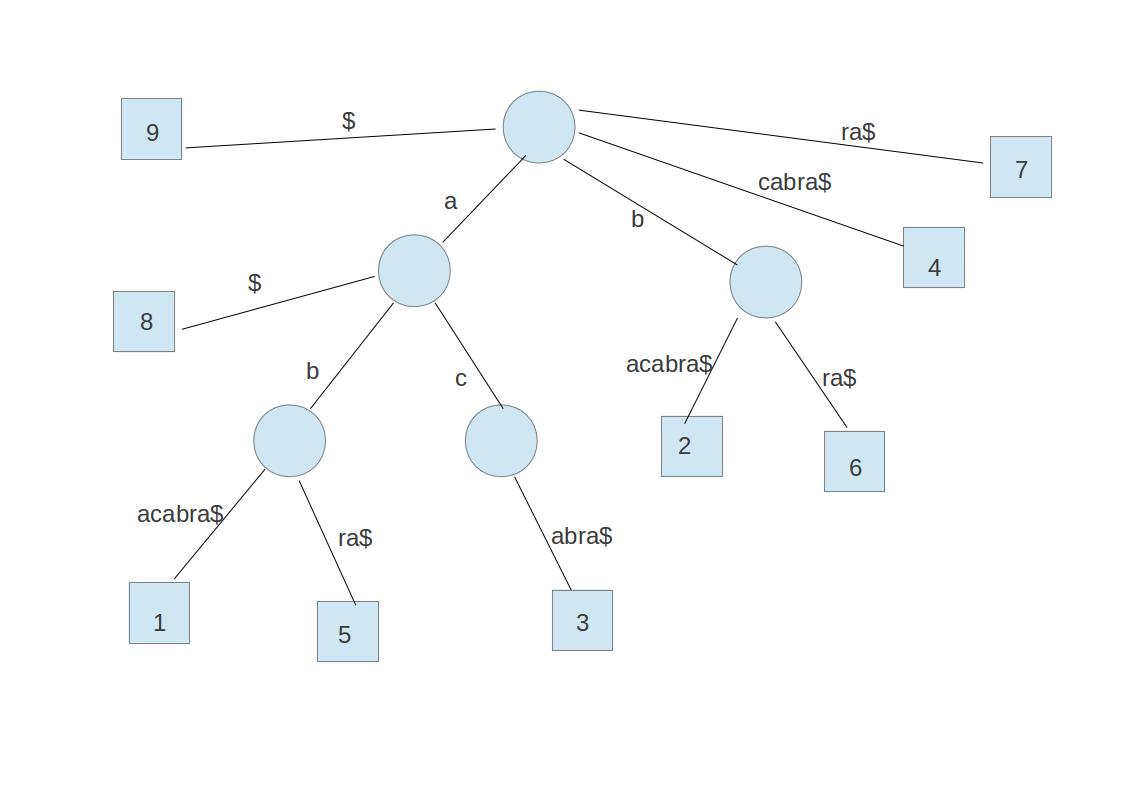
\includegraphics[scale=0.28]{SuffixTree.jpg}
\end{figure}
\end{itemize}
\end{frame}

\begin{frame}
\frametitle{Cluster Eigenschaft und Longest Common Prefix}
\begin{itemize}
\item Such Intervall entpsricht Teilbaum
\item Im Such Intervall \textit{kann} es also LCPs geben: \color{red}rosa\color{black}: ''ab", mit \color{purple}lila \color{black}:''a", mit \color{green}grün\color{black}: kein LCP
\begin{figure}[hbtp]
\centering
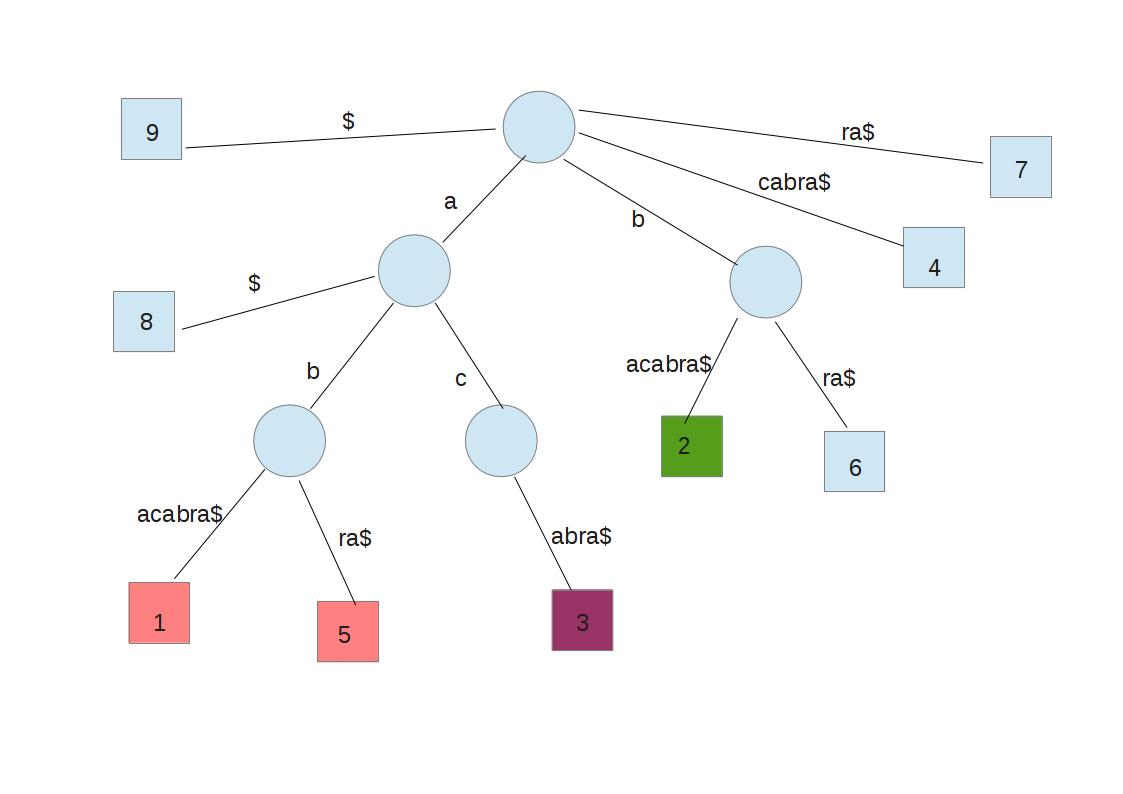
\includegraphics[scale=0.28]{SuffixTreeLCP.jpg}
\end{figure}

\end{itemize}
\end{frame}

\begin{frame}
\frametitle{Suffix Array und Longest Common Prefix}
\begin{itemize}
\item Sei S ein Such Intervall [O,U], $M = \lfloor \frac{O+U}{2}\rfloor$ = Treffer
\item Wir definieren zwei LCPs: oben = $LCP(T_{A[O],n},T_{A[M],n})$ und unten = $LCP(T_{A[M],n},T_{A[U],n}))$
\item Bei sequenzieller Suche nur Vergleich von $T_{A[i]+\vert oben\vert, A[i]+m}$ nötig
\end{itemize}
\end{frame}
%%%%%%%%5     Bsp. Anna_Annanas
\begin{frame}
\frametitle{Bsp. p = ''anna'' in T = ''annanas\_anna\$''}
\begin{tabular}{l|l<{\ttfamily}}
\textbf{A[i]} & $T_{A[i],n}$\\\hline
13 & \$\\
8 & \_anna\$\\
12 & a\$\\
4 & anas\_anna\$\\
9 & anna\$\\
1 & annanas\_anna\$\\
6 & \color{red}as\_a\color{black}\_nna\$ ''anna'' < \color{red}''as\_a''\color{black}$\rightarrow$ obere Hälfte\\%MMMMMMMMMMMM
11 & na\$\\
3 & nanas\_anna\$\\
5 & nasanna\$\\
10 & nna\$\\
2 & nnanas\_anna\$\\
7 & s\_anna\$\\
\end{tabular}
\end{frame}

\begin{frame}
\frametitle{Bsp. p = ''anna'' in T = ''annanas\_anna\$''}
\begin{tabular}{l|l<{\ttfamily}}
\textbf{A[i]} & $T_{A[i],n}$\\\hline
13 & \$\\
8 & \_anna\$\\
12 & a\$\\
4 & \color{red}anas\color{black}\_anna\$ ''anna'' > \color{red}''anas''\color{black}$\rightarrow$ untere Hälfte\\ %MMMMMMMMMM
9 & anna\$\\
1 & annanas\_anna\$\\
6 & as\_anna\$ \\
11 & \color{gray}na\$\\
3 & \color{gray}nanas\_anna\$\\
5 & \color{gray}nasanna\$\\
10 & \color{gray}nna\$\\
2 & \color{gray}nnanas\_anna\$\\
7 & \color{gray}s\_anna\$\\
\end{tabular}
\end{frame}

\begin{frame}
\frametitle{Bsp. p = ''anna'' in T = ''annanas\_anna\$''}
\begin{tabular}{l|l<{\ttfamily}}
\textbf{A[i]} & $T_{A[i],n}$\\\hline
13 & \color{gray}\$\\
8 & \color{gray}\_anna\$\\
12 & \color{gray}a\$\\
4 & anas\_anna\$ \\
9 & anna\$ \\ %MMMMMMMMMM
1 & \color{red}anna\color{black}nas\_anna\$ ''anna'' == \color{red}''anna''\color{black}$\rightarrow$ Treffer!\\
6 & as\_anna\$ \\
11 & \color{gray}na\$\\
3 & \color{gray}nanas\_anna\$\\
5 & \color{gray}nasanna\$\\
10 & \color{gray}nna\$\\
2 & \color{gray}nnanas\_anna\$\\
7 & \color{gray}s\_anna\$\\
\end{tabular}
\begin{itemize}
\item oben = LCP(''anna\$'', ''anas\_anna\$'') = ''an''
\item unten = LCP(''anna\$'', ''as\_anna\$'') = ''a''
\end{itemize}
\end{frame}

\begin{frame}
\frametitle{Sequenzielle Suche mit LCP}
\begin{itemize}
\item nach unten, normal: ''anna'' $\neq$ ''as\_a'', 4 Zeichenvergleiche
\item nach unten, mit LCP: ''\color{gray}a\color{red}nna'' $\neq$ ''\color{gray}a\color{red}s\_a\color{black}'', 3 Zeichenvergleiche
\item nach oben, normal: ''anna'' == ''anna'', 4 Zeichenvergleiche
\item nach oben, mit LCP: ''\color{gray}an\color{red}na'' == ''\color{gray}an\color{red}na\color{black}'', 2 Zeichenvergleiche
\item nach oben, normal: ''anna'' $\neq$ ''anas'', 4 Zeichenvergleiche
\item nach oben, mit LCP: ''\color{gray}an\color{red}na'' $\neq$ ''\color{gray}an\color{red}as\color{black}'', 2 Zeichenvergleiche
\end{itemize}
\end{frame}

\begin{frame}
\frametitle{Zwischen-Resultat}
\begin{itemize}
\item Such Intervalle \textit{können} längste gemeinsame Präfixe besitzen
\item Im schlechtesrn Fall kein LCP $\rightarrow$ keine Laufzeitverbesserung
\item In der Praxis aber schneller als nur binäre Suche.
\end{itemize}
\end{frame}
%%%%%%%%%%%%%% SA-Complex:
\begin{frame}
\frametitle{Weitere Verbesserungen durch LCPs}
\begin{itemize}
\item Vorausberechnung aller 2n-3 Suchintervalle [L,R] wobei L<R
\item Berechnung des LCP für jedes dieser Intervalle
\end{itemize}
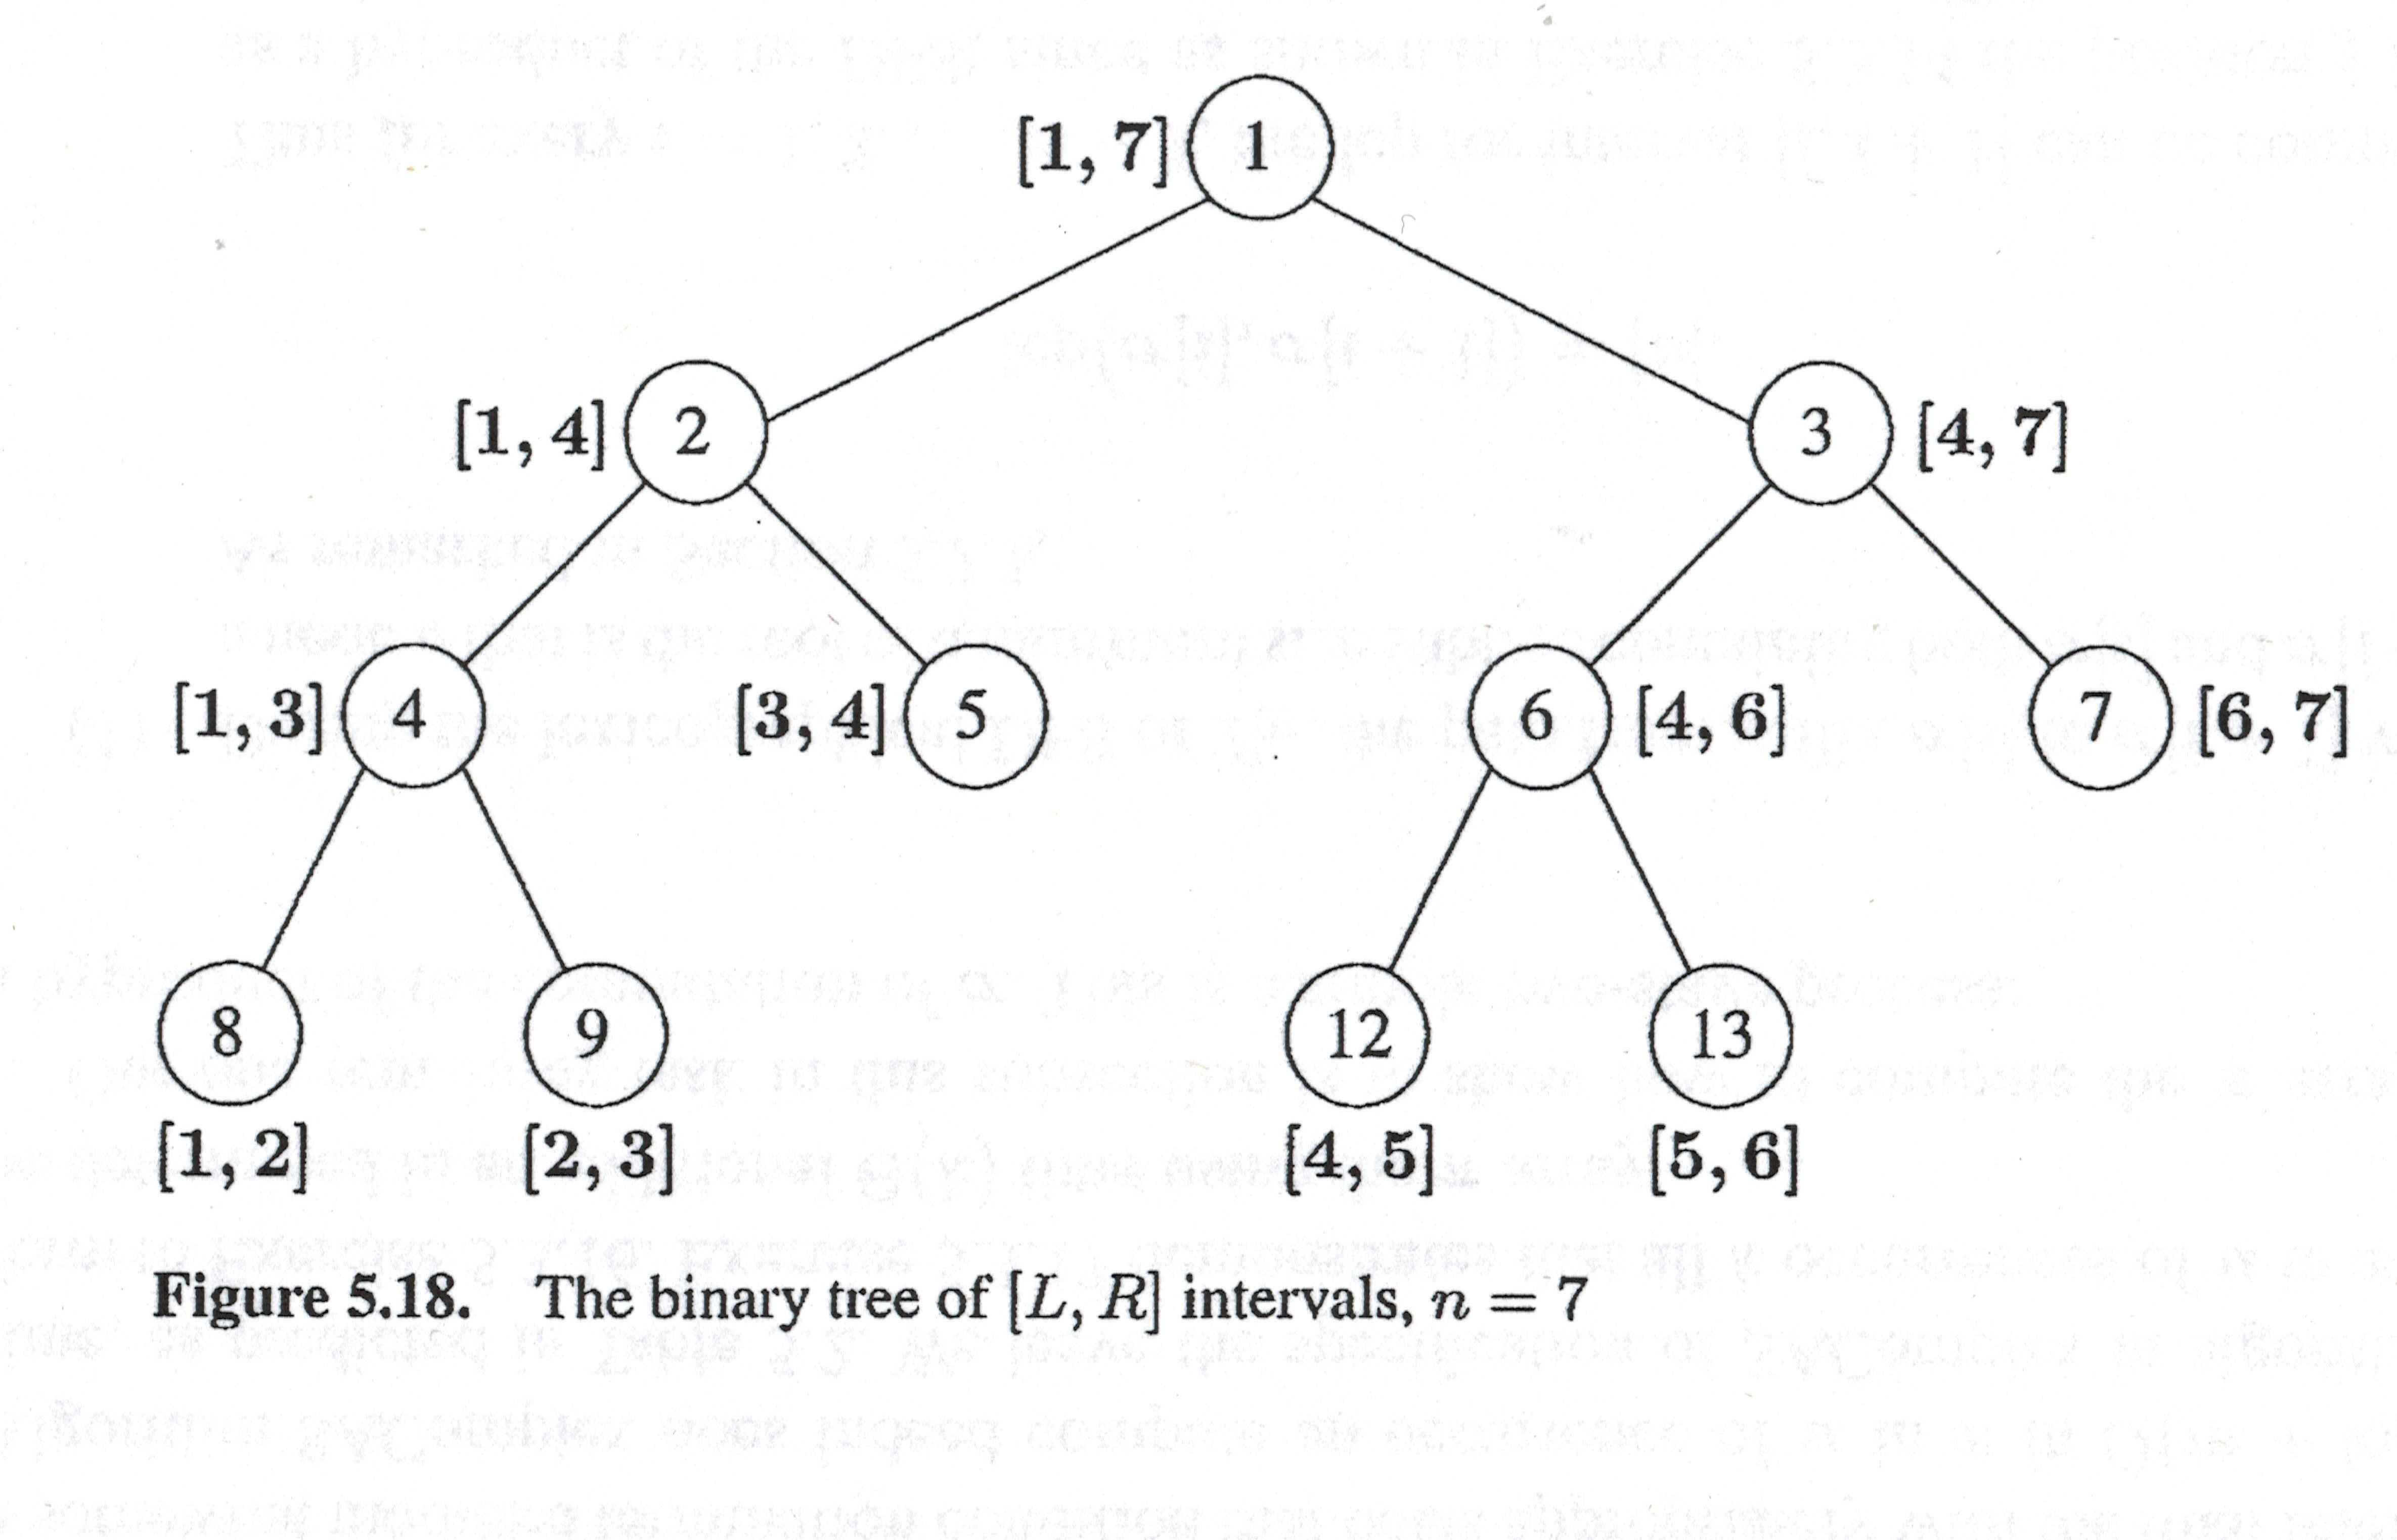
\includegraphics[scale=1]{intervalle.jpeg}
\end{frame}

\begin{frame}
\frametitle{LCP-Array $\pi$}
\begin{itemize}
\item Für jedes Suchintervall [L,R] gibt es genau ein lcp($T_{A[R],n}$,$T_{A[L],n}$)
\item Wird in LCP-Array $\pi$ abgespeichert, max. Dimension 3n-8
\item $\pi$ ist Nebenprodukt bei Berechnung von Suffix Array A, falls Herleitung aus Suffix Tree
\end{itemize}
\end{frame}

\begin{frame}
\frametitle{LCP Array $\pi$}
Es seien $P_L = lcp(p,T_{A[L],n}$) und $P_{LM} = lcp(T_{A[M],n},T_{A[L],n}) = \pi[i]$, dann gibt es 3 Fälle:\newline
\begin{enumerate}
\item $P_{LM} > P_L$: Pattern p kann \textit{nicht} in [L,M] liegen ($\rightarrow$ Cluster Eigenschaft), wenn dann in [M,R]
\item $P_{LM} < P_L$: p liegt wenn dann in [L,M], sicher \textit{nicht} in [M,R]
\item $P_{LM} = P_L$: Vergleiche p mit $T_{A[M],A[M]+m}$ falls <0 $\rightarrow$ nach links, >0 $\rightarrow$ nach rechts, ==0 Treffer
\end{enumerate}
\end{frame}

\begin{frame}
\frametitle{Zusammenfassung: Binäre Suche in Suffix Arrays}
\begin{itemize}
\item Finden der n Suffixes in T: $\mathcal{O}(n)$ und lexikografisch Sortieren: $\mathcal{O}(n\cdot log (n))$
\item Auch in $\mathcal{O}(n)$ möglich
\item Binäre Suche mit LCP: $\mathcal{O}(m\cdot (k + log(n)))$
\item Binäre Suche mit berechneten Suchintervallen und LCP-Array: $\mathcal{O}(m + k + log(n))$
\end{itemize}
\end{frame}
%%%%%  Backward Search
\subsection{Backward Search}
\begin{frame}
\frametitle{Backward Search}
\begin{itemize}
\item Grundlage: Suffix Array
\item Neu: keine binäre Suche, finden von zB \glqq b\grqq mit Array C[\glqq b\grqq ] = 5
\item Vorheriger Buchstabe $T_{A[i]-1}$ des Suffix $T_{A[i],n}$
\end{itemize}
\end{frame}

\begin{frame}
\frametitle{Bsp.: Suche von p = \glqq abra\grqq }
T = \glqq abacabra\$\grqq\\[5mm]
\begin{tabular}{l<{\ttfamily}|c<{\ttfamily} c<{\ttfamily}c<{\ttfamily} l<{\ttfamily}}
\textbf{i} & $A[i]$ & $T_{A[i]-1}$ & $T_{A[i],n}$\\\hline
1 & 9 & a & \$ \\
2 & 8 & r & a\$ \\
3 & 1 & \$ & abacabra\$ \\
4 & 5 & c & abra\$ \\
5 & 3 & b & acabra\$ \\
6 & 2 & a & bacabra\$ \\
7 & 6 & a & bra\$ \\
8 & 4 & a & cabra\$ \\
9 & 7 & b & ra\$ \\
\end{tabular}\\[5mm]
\begin{itemize}
\item \glqq abr{\color{red}\textbf{a}}\grqq von hinten: alle \texttt{a}, von C[\glqq a\grqq ]+1 bis C[\glqq b\grqq ]
\end{itemize}
\end{frame}
\begin{frame}
\frametitle{Bsp.: Suche von p = \glqq abra\grqq (Schritt 1)}
\begin{itemize}
\item Darunter alle \glqq a\grqq mit Vorgänger \glqq r\grqq\\[5mm]
\begin{tabular}{l<{\ttfamily}|c<{\ttfamily} c<{\ttfamily}c<{\ttfamily} l<{\ttfamily}}
\textbf{i} & $A[i]$ & $T_{A[i]-1}$ & $T_{A[i],n}$\\\hline
1 & 9 & a & \$ \\
\textbf{2} & \textbf{8} & \color{red}\textbf{r} & \textbf{a\$} \\
3 & 1 & \$ & abacabra\$ \\
4 & 5 & c & abra\$ \\
5 & 3 & b & acabra\$ \\
6 & 2 & a & bacabra\$ \\
7 & 6 & a & bra\$ \\
8 & 4 & a & cabra\$ \\
9 & 7 & b & ra\$ \\
\end{tabular}\\[5mm]
\item Weiter zu i = C[\glqq r\grqq]+1 = 9
\end{itemize}
\end{frame}
\begin{frame}
\frametitle{Bsp.: Suche von p = \glqq abra\grqq (Schritt 2)}
\begin{itemize}
\item Suche \glqq a\color{red}\textbf{b}\color{black}ra\grqq in r mit Vorgänger b
\begin{tabular}{l<{\ttfamily}|c<{\ttfamily} c<{\ttfamily}c<{\ttfamily} l<{\ttfamily}}
\textbf{i} & $A[i]$ & $T_{A[i]-1}$ & $T_{A[i],n}$\\\hline
1 & 9 & a & \$ \\
2 & 8 & r & a\$ \\
3 & 1 & \$ & abacabra\$ \\
4 & 5 & c & abra\$ \\
5 & 3 & \color{red}b \color{black}& acabra\$ \\
6 & 2 & a & bacabra\$ \\
7 & 6 & a & bra\$ \\
8 & 4 & a & cabra\$ \\
\textbf{9} & \textbf{7} & \color{red}\textbf{b} & \textbf{ra\$} \\
\end{tabular}\\[5mm]
\item b ist bei i = 5 bereits \textit{einmal} in $T_{A[i]-1}$ vorgekommen \textrightarrow suche von C[\glqq b\grqq]+1\textit{+1} bis C[\glqq c\grqq], d.h. bei i = 7
\item Problem: z.B. \textit{wie oft ist \glqq b\grqq  in Spalte $T_{A[i]-1}$ vor i = 5} erfordert lineares Durchsuchen von $T_{A[i]-1}\ \rightarrow\ \mathcal{O}(m\cdot n)$.
\end{itemize}
\end{frame}

%%%%%%% Occ Funktion

\begin{frame}
\frametitle{Lösung: Funktion Occ(c,i)}
\begin{itemize}
\item Für alle c aus $\Sigma$ sei $B^{c}$ ein Bit-Vektor mit $B^{c}[i] = 1$ falls $T_{A[i]-1} = c$
\item Eine weitere Funktion $rank_{b}(B,i)$ liefert die Anzahl von zB b=1 in B vor i, s.d $rank_{1}(B^{c},i) = Occ(c,i)$.
\item Dies benötigt linear mehr Speicher, doch der Zugriff durch rank ist konstant, s.d. $\mathcal{O}(m)$ insgesamt garantiert ist.
\end{itemize}
\end{frame}
\begin{frame}
\frametitle{Bsp.: Suche von p = \glqq abra\grqq (Schritt 3)}
\begin{itemize}
\item Finde alle \glqq{\color{red}\textbf{a}}bra\grqq  in b mit Vorgänger \glqq a\grqq:\\[5mm]
\begin{tabular}{l<{\ttfamily}|c<{\ttfamily} c<{\ttfamily}c<{\ttfamily} l<{\ttfamily}}
\textbf{i} & $A[i]$ & $T_{A[i]-1}$ & $T_{A[i],n}$\\\hline
1 & 9 & \color{red}a \color{black}& \$ \\
2 & 8 & r & a\$ \\
3 & 1 & \$ & abacabra\$ \\
4 & 5 & c & abra\$ \\
5 & 3 & b & acabra\$ \\
6 & 2 & \color{red}a & \color{black}bacabra\$ \\
\textbf{7} & \textbf{6}  & \color{red}\textbf{a} & \textbf{bra\$} \\
8 & 4 & a & cabra\$ \\
9 & 7 & b & ra\$ \\
\end{tabular}\\[5mm]
\item Occ(''a'', 7) = 2 \textrightarrow suche von C[\glqq a\grqq]+1\textit{+2} bis C[\glqq b\grqq], d.h. bei i = 4
\end{itemize}
\end{frame}
\begin{frame}
\frametitle{Bsp.: Suche von p = \glqq abra\grqq  (Schritt 4)}
\begin{tabular}{l<{\ttfamily}|c<{\ttfamily} c<{\ttfamily}c<{\ttfamily} l<{\ttfamily}}
\textbf{i} & $A[i]$ & $T_{A[i]-1}$ & $T_{A[i],n}$\\\hline
1 & 9 & a & \$ \\
2 & 8 & r & a\$ \\
3 & 1 & \$ & abacabra\$ \\
4 & 5 & c & \color{red}\textbf{abra\$} \\
5 & 3 & b & acabra\$ \\
6 & 2 & a & bacabra\$ \\
7 & 6 & a & bra\$ \\
8 & 4 & a & cabra\$ \\
9 & 7 & b & ra\$ \\
\end{tabular}\\[5mm]
\begin{itemize}
\item Nach 4 Schritten (= Länge m von p) ist das Pattern gefunden $\rightarrow \mathcal{O}(m)$
\end{itemize}
\end{frame}
%%%%%%%%%%%%%%%% Forward Searching
\begin{frame}
\subsection{Forward Searching}
\frametitle{Forward Searching}
\begin{itemize}
\item Vorherige Position: $LF(i) = C[T_{A[i]-1}] + Occ(T_{A[i]-1},i)$
\item Während beim Backward Searching ein Suffix auf das vorhergehende abgebildet wird, ist es hier umgekehrt
\item Inverse Funktion $\Psi(i) = i'$, s.d. A[i'] = (A[i] mod n)+1 bildet die Pos. eines Suffix auf die seines Nachfolgers ab
\end{itemize}
\end{frame}
\begin{frame}
\frametitle{Bsp.: $\Psi$ zu T = \glqq abacabra\$\grqq}
\begin{tabular}{l<{\ttfamily}|c<{\ttfamily} c<{\ttfamily}c<{\ttfamily} c<{\ttfamily}c<{\ttfamily}c<{\ttfamily} r<{\ttfamily}}
i & $A[i]$ & $\Psi$ & newF & $T_{A[i],n}$ \\\hline
1 & 9 & 3 & 1 &\$\\
2 & 8 & 1 & 1 &a\$\\
3 & 1 & 6 & 0 &abacabra\$\\
4 & 5 & 7 & 0 &abra\$\\
5 & 3 & 8 & 0 &acabra\$\\
6 & 2 & 5 & 1 &bacabra\$\\
7 & 6 & 9 & 0 &bra\$\\
8 & 4 & 4 & 1 &cabra\$\\
9 & 7 & 2 & 1 &ra\$\\
\end{tabular}
\end{frame}
\begin{frame}
\frametitle{Suche von p in T}
\begin{itemize}
\item Falls $\forall c: c \in \Sigma \Rightarrow c \in T$ ex. $\sigma$ aufsteigende Zahlenfolgen in $\Psi$: 3; 1,6,7,8; 5,9; 4; 2;
\item Diese zeigen an, wo sich der erste Buchstabe des Suffix ändert. Als Bitvektor newF = 110001011
\item Die Suche von p erfolgt binär, wobei p ein Prefix des jew. Suffix ist, welches durch rekursives Folgen von $\Psi(i)$ \textit{ohne das Suffix Array} gefunden werden kann
\item Der jew. erste Buchstabe $T_{A[i]}$ des Suffixes $T_{A[i],n}$ wird durch $rank_1(newF,i)$ ermittelt. Falls zB $rank_1(newF,i) = 2$ ist c = \glqq a\grqq.
\end{itemize}
\end{frame}

\begin{frame}
\frametitle{Bsp: p = ''aba'' in ''abacabra\$''}
\begin{itemize}
\item $rank_1(newF, 5) = 2 \rightarrow$ erster Buchstabe: ''a''
\end{itemize}
\begin{tabular}{l<{\ttfamily}|c<{\ttfamily}c<{\ttfamily} r<{\ttfamily}}
i & $\Psi$ & newF & $T_{A[i],n}$ \\\hline
1 & 3 & 1 &\$\\
2 & 1 & 1 &a\$\\
3 & 6 & 0 &abacabra\$\\
4 & 7 & 0 &abra\$\\
5 & 8 & 0 & ''\color{red}a\color{gray}ba\color{black}'' == \color{red}a\color{gray}cabra\$\\
6 & 5 & 1 &bacabra\$\\
7 & 9 & 0 &bra\$\\
8 & 4 & 1 &cabra\$\\
9 & 2 & 1 &ra\$\\
\end{tabular}
\end{frame}

\begin{frame}
\frametitle{Bsp: p = ''aba'' in ''abacabra\$''}
\begin{itemize}
\item $rank_1(newF, \Psi(5)) = rank_1(newF, 8) = 4 \rightarrow$ nächster Buchstabe: ''c''
\end{itemize}
\begin{tabular}{l<{\ttfamily}|c<{\ttfamily}c<{\ttfamily} r<{\ttfamily}}
i & $\Psi$ & newF & $T_{A[i],n}$ \\\hline
1 & 3 & 1 &\$\\
2 & 1 & 1 &a\$\\
3 & 6 & 0 &abacabra\$\\
4 & 7 & 0 &abra\$\\
5 & 8 & 0 & ''\color{red}ab\color{gray}a\color{black}'' < \color{red}ac\color{gray}abra\$\\
6 & 5 & 1 &bacabra\$\\
7 & 9 & 0 &bra\$\\
8 & 4 & 1 &cabra\$\\
9 & 2 & 1 &ra\$\\
\end{tabular}
\end{frame}

\begin{frame}
\frametitle{Bsp: p = ''aba'' in ''abacabra\$''}
\begin{itemize}
\item $rank_1(newF, 3) = 2 \rightarrow$ erster Buchstabe: ''a''
\end{itemize}
\begin{tabular}{l<{\ttfamily}|c<{\ttfamily}c<{\ttfamily} r<{\ttfamily}}
i & $\Psi$ & newF & $T_{A[i],n}$ \\\hline
1 & 3 & 1 &\$\\
2 & 1 & 1 &a\$\\
3 & 6 & 0 &''\color{red}a\color{gray}ba\color{black}'' == \color{red}a\color{gray}bacabra\$\\
4 & 7 & 0 &abra\$\\
5 & 8 & 0 & acabra\$\\
\color{gray}6 & \color{gray}5 & \color{gray}1 &\color{gray}bacabra\$\\
\color{gray}7 & \color{gray}9 & \color{gray}0 &\color{gray}bra\$\\
\color{gray}8 &\color{gray} 4 & \color{gray}1 &\color{gray}cabra\$\\
\color{gray}9 & \color{gray}2 & \color{gray}1 &\color{gray}ra\$\\
\end{tabular}
\end{frame}

\begin{frame}
\frametitle{Bsp: p = ''aba'' in ''abacabra\$''}
\begin{itemize}
\item $rank_1(newF, \Psi(3)) = rank_1(newF, 6) = 3 \rightarrow$ nächster Buchstabe: ''b''
\end{itemize}
\begin{tabular}{l<{\ttfamily}|c<{\ttfamily}c<{\ttfamily} r<{\ttfamily}}
i & $\Psi$ & newF & $T_{A[i],n}$ \\\hline
1 & 3 & 1 &\$\\
2 & 1 & 1 &a\$\\
3 & 6 & 0 &''\color{red}ab\color{gray}a\color{black}'' == \color{red}ab\color{gray}acabra\$\\
4 & 7 & 0 &abra\$\\
5 & 8 & 0 & acabra\$\\
\color{gray}6 & \color{gray}5 & \color{gray}1 &\color{gray}bacabra\$\\
\color{gray}7 & \color{gray}9 & \color{gray}0 &\color{gray}bra\$\\
\color{gray}8 &\color{gray} 4 & \color{gray}1 &\color{gray}cabra\$\\
\color{gray}9 & \color{gray}2 & \color{gray}1 &\color{gray}ra\$\\
\end{tabular}
\end{frame}

\begin{frame}
\frametitle{Bsp: p = ''aba'' in ''abacabra\$''}
\begin{itemize}
\item $rank_1(newF, \Psi(6)) = rank_1(newF, 5) = 2 \rightarrow$ nächster Buchstabe: ''a''
\end{itemize}
\begin{tabular}{l<{\ttfamily}|c<{\ttfamily}c<{\ttfamily} r<{\ttfamily}}
i & $\Psi$ & newF & $T_{A[i],n}$ \\\hline
1 & 3 & 1 &\$\\
2 & 1 & 1 &a\$\\
3 & 6 & 0 &''\color{red}aba\color{black}'' == \color{red}aba\color{gray}cabra\$\\
4 & 7 & 0 &abra\$\\
5 & 8 & 0 & acabra\$\\
\color{gray}6 & \color{gray}5 & \color{gray}1 &\color{gray}bacabra\$\\
\color{gray}7 & \color{gray}9 & \color{gray}0 &\color{gray}bra\$\\
\color{gray}8 &\color{gray} 4 & \color{gray}1 &\color{gray}cabra\$\\
\color{gray}9 & \color{gray}2 & \color{gray}1 &\color{gray}ra\$\\
\end{tabular}
\end{frame}

\begin{frame}
\frametitle{Fazit Forward Searching}
\begin{itemize}
\item $\Psi$ ersetzt A[i].
\item Weder A[i] noch T sind zur Suche von p in T nötig
\item $\Psi$ kann durch \textit{gap-encoding} weiter komprimiert werden.
\end{itemize}
\end{frame}

\begin{frame}
\frametitle{Zusammenfassung Backward- und Forward Suche}
\begin{itemize}
\item \textbf{Backward Suche:} Zusätzliche Hilfsfunktion $LF(i) = C[T_{A[i]-1}] + Occ(T_{A[i]-1},i)$ nötig, mehr Speicherbederf, aber in $\mathcal{O}(k \cdot m)$ Zeit.
\item \textbf{Forward Suche:} $\mathcal{O}(k \cdot m \cdot log(n))$ Zeit, aber $\Psi$ reicht aus, T, A nicht nötig $\rightarrow$ Self index
\end{itemize}
\end{frame}

\section{Burrows-Wheeler Transformation}
\begin{frame}
\frametitle{Burrows-Wheeler Transformation}
\begin{itemize}
\item Die BWT ist eine Permutation von T, s.d. an jeder Stelle des Suffix Arrays der vorherige Buchstabe angehängt wird:
\end{itemize}
\begin{Definition}
Sei $T_{1,n}$ ein String und A[1,n] sein Suffix Array. Dann ist die BWT $T_{1,n}^{bwt}$ von T: \newline $T_{i}^{bwt} = T_{A[i]-1}$ $\forall 1 \leq i \leq n$ ausser A[i] = 1 $\Rightarrow$ $T_{i}^{bwt} = T_n = \$ $
\end{Definition}
\end{frame}
\begin{frame}
\frametitle{Anschauliches Beispiel, T = \glqq abacabra\$\grqq}
\begin{tabular}{l<{\ttfamily} c<{\ttfamily} r<{\ttfamily}}
\textbf{Permutationen} & \textbf{lex. geordnet} & $F\ldots L = T^{bwt}$ \\\hline
abacabra\$ & \$abacabra & \$...a \\
bacabra\$a & a\$abacabr & a...r \\
acabra\$ab & abacabra\$ & a...\$ \\
cabra\$aba & abra\$abac & a...c \\
abra\$abac & acabra\$ab & a...b \\
bra\$abaca & bacabra\$a & b...a \\
ra\$abacab & bra\$abaca & b...a \\
a\$abacabr & cabra\$aba & c...a \\
\$abacabra & ra\$abacab & r...b \\
\end{tabular}\\[5mm]
\end{frame}

\begin{frame}
\frametitle{Anschauliches Beispiel, T = \glqq abacabra\$\grqq}
\begin{tabular}{l<{\ttfamily} |c<{\ttfamily} |cc<{\ttfamily}| r<{\ttfamily}}
\textbf{Permutationen} & \textbf{Suffix Array} & A[i] & $F\ldots L = T^{bwt}$ \\\hline
abacabra\$ & \$\color{gray}abacabra &9& \$...a \\
bacabra\$\color{gray}a & a\$\color{gray}abacabr &8& a...r \\
acabra\$\color{gray}ab & abacabra\$ & 1&a...\$ \\
cabra\$\color{gray}aba & abra\$\color{gray}abac &5& a...c \\
abra\$\color{gray}abac & acabra\$\color{gray}ab &3& a...b \\
bra\$\color{gray}abaca & bacabra\$\color{gray}a & 2&b...a \\
ra\$\color{gray}abacab & bra\$\color{gray}abaca &6& b...a \\
a\$\color{gray}abacabr & cabra\$\color{gray}aba & 4&c...a \\
\$\color{gray}abacabra & ra\$\color{gray}abacab &7& r...b \\
\end{tabular}\\[5mm]
\begin{itemize}
\item $T^{bwt}$ = ar\$cbaaab
\item BWT Permutation besser für weitere Komprimierung von T als T selbst
\end{itemize}
\end{frame}

% Zusammenfassung
\begin{frame}
\frametitle{Zusammenfassung und Fragen}
\begin{itemize}
\item Suffix Arrays und Zusammenhang mit Suffix Trees
\item Binäre Suche mit LCP
\item Backward- und Forward Suche
\item Suffix Arrays in der BWT
\end{itemize}
\textbf{Vielen Dank für Eure Aufmerksamkeit!}
\end{frame}

\end{document}